%----------------------------------------------------------------------------------------
%	PACKAGES AND OTHER DOCUMENT CONFIGURATIONS
%----------------------------------------------------------------------------------------

%---
% TOOlS: 
% To convert jpg, png to pdf use: convert *.jpg *.pdf
%-----

\documentclass[letterpaper, 10pt]{article} % A4 paper size and default 11pt font size

\usepackage[utf8]{inputenc} % Required for inputting international characters
\usepackage[spanish,es-tabla]{babel}
\usepackage[T1]{fontenc} % Output font encoding for international characters
\usepackage{stix} % Use the STIX fonts
\usepackage{listings}
\usepackage[left=3cm]{geometry}
\usepackage[final]{pdfpages}
\usepackage{graphicx}
\usepackage{hyperref}
\usepackage{float}
\usepackage{amsmath}
\usepackage{pdfpages}


% Comandos

\renewcommand{\lstlistingname}{Código}
\renewcommand{\lstlistlistingname}{Índice de fragmentos de código fuente}
\newcommand{\grad}{$^{\circ}$}

\title{Memoria descriptiva estación de radioaficionado}
\author{EA4HDO. Juan Alberto Agudo Huertas}


\begin{document}

%%----------------------------------------------------------------------------------------
%%	TITLE PAGE
%%----------------------------------------------------------------------------------------

\begin{titlepage} % Suppresses displaying the page number on the title page and the subsequent page counts as page 1
	
	\raggedleft % Right align the title page
	
	\rule{1pt}{\textheight} % Vertical line
	\hspace{0.05\textwidth} % Whitespace between the vertical line and title page text
	\parbox[b]{0.90\textwidth}{ % Paragraph box for holding the title page text, adjust the width to move the title page left or right on the page
		
		{\Huge\bfseries Memoria descriptiva \\[0.5\baselineskip] Estación radioaficionado}\\[2\baselineskip] % Title
		{\large\textit{Titular: EA4HDO \\ versión documento: 0 [Primera instalación] }}\\[4\baselineskip] % Subtitle or further description
		{\Large\textsc{Juan Alberto Agudo Huertas}} % Author name, lower case for consistent small caps
		
		\vspace{0.5\textheight} % Whitespace between the title block and the publisher
		
		{\noindent En Madrid a 09 Febrero de 2020}\\[\baselineskip] % Ref Date
	}

\end{titlepage}

%----------------------------------------------------------------------------------------

\tableofcontents

\newpage

\section{Ubicación de la casa y descripción de los elementos cercanos.}
El sistema radiante se ubicará en la finca n33 de la calle de los morales, 28054 Madrid. Sobre el tejado de un edificio de 6 plantas más ático. La estación de radio se situan en el piso 3 letra D bloque B.
%\includepdf[pages=-]{img/morales1.pdf}

\begin{figure}[h!]
\centering
\includegraphics[trim = 8mm 47mm 110mm 47mm, clip, width=10cm]{img/morales2.pdf}
\caption{C. Los morales 29-35 Bloque B vista frontal entrada por el portal }
\label{fig:morales1}
\end{figure}

\begin{figure}[h!]
\centering
\includegraphics[trim = 8mm 47mm 110mm 47mm, clip, width=10cm]{img/morales4.pdf}
\caption{C. Los morales 29-35 Bloque B vista trasera del portal}
\label{fig:morales2}
\end{figure}

\begin{figure}[h!]
\centering
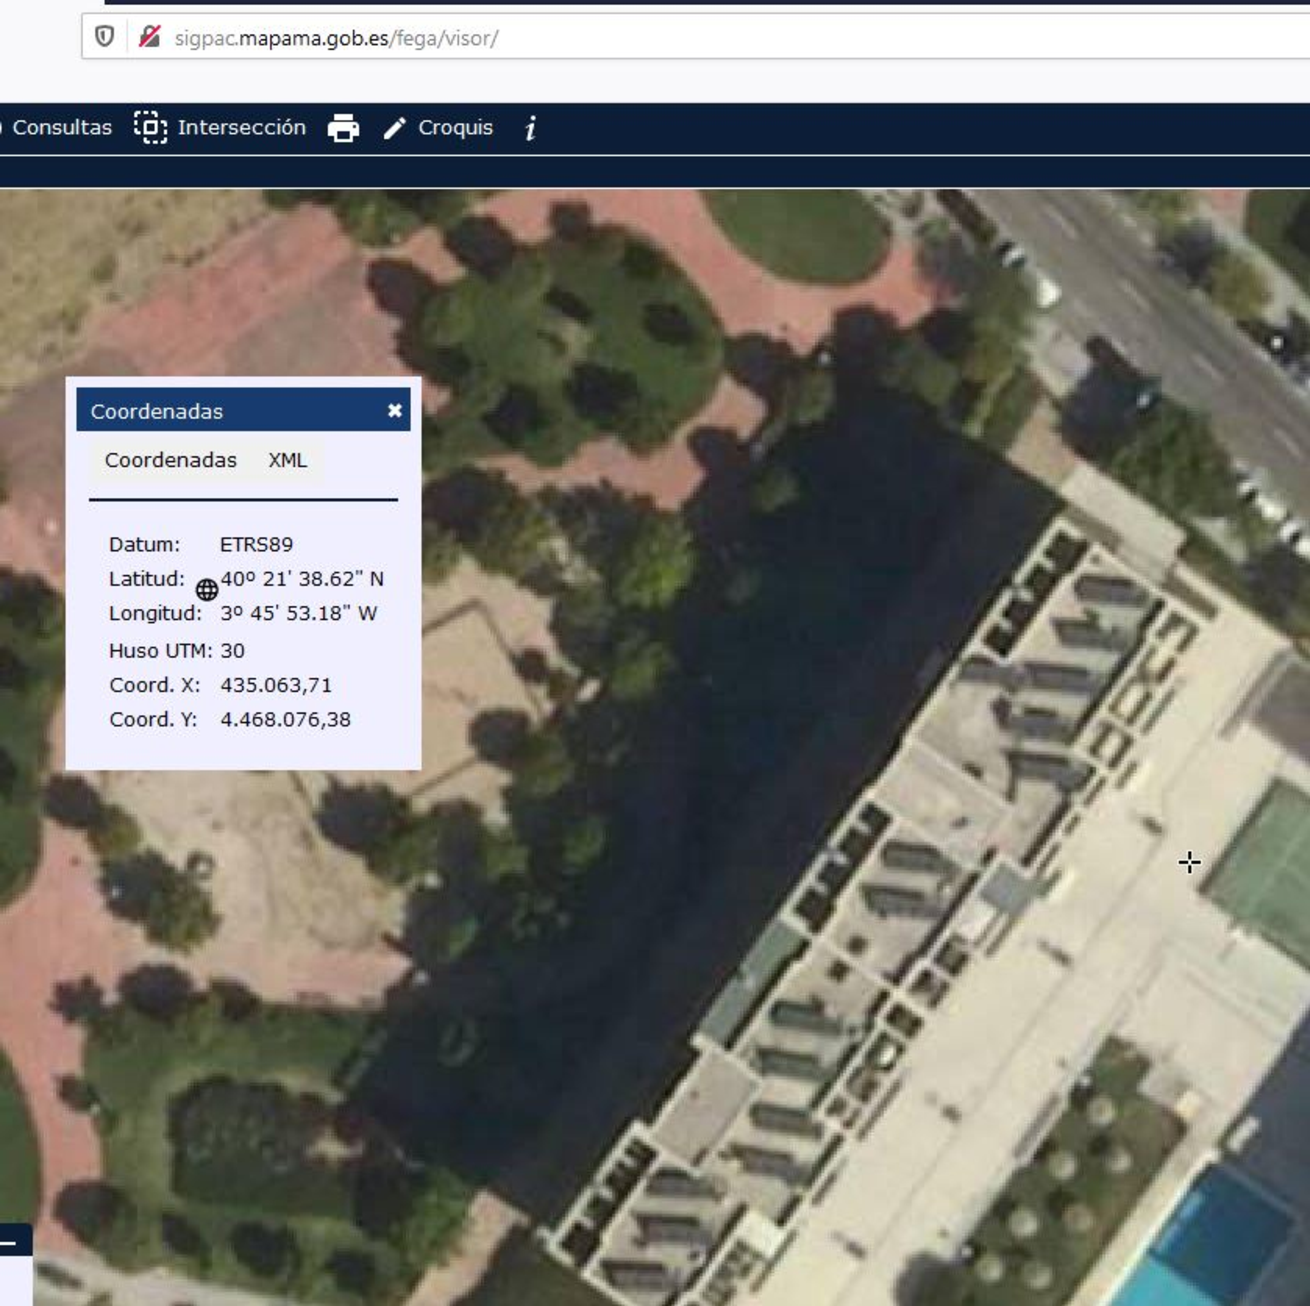
\includegraphics[width=10cm]{img/sigpac.pdf}
\caption{Captura de Sigpac}
\label{fig:sigpac}
\end{figure}

Coordenadas:\\
\\
Datum: ETRS89 \\
Latitud: 40\grad 21' 38.62'' N \\
Longitud: 3\grad 45' 53.18'' W \\
Huso UTM: 30 \\
Coord. X: 435.063,71 \\
Coord Y: 4.468.076,38 \\



\newpage

\section{Ubicación de las antenas en el tejado y los puntos de anclaje.}
En el siguiente esquema se indica la ubicación aproximada de las antenas en el tejado.La instalación conlleva una antena vertical y dos dipolos simples.
\begin{figure}[h!]
\centering
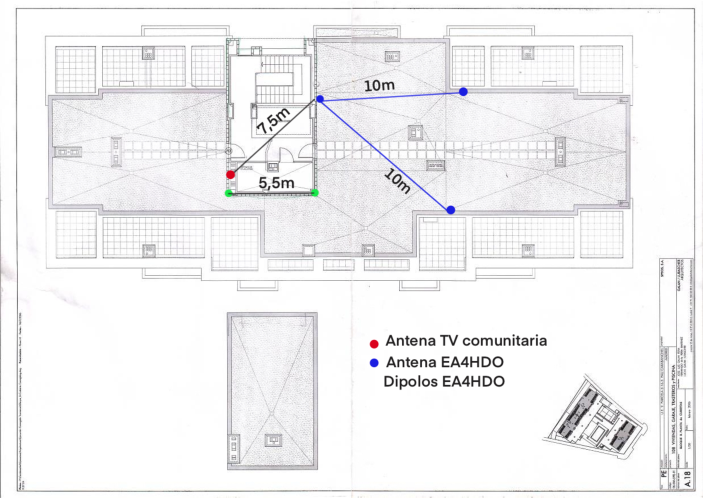
\includegraphics[clip, width=17cm]{img/planoAntenas.pdf}
\caption{Esquema antenas EA4HDO}
\label{fig:esquema}
\end{figure}

\subsection{Mástil}
En color azul se indica la posición del mástil de 3 metros en el cual se instalará la antena vertical para VHF, UHF, antena discono y dipolo multibanda. 
El mástil que se instalará es un televes referencia 301003, \url{https://www.televes.com/es/301003-mastil-3m-x-o-45mm-x-espesor-2mm.html}, 45mm de diametro y 2mm de espesor como se puede ver en la figura \ref{fig:mastil}

\begin{figure}[h!]
	\centering
	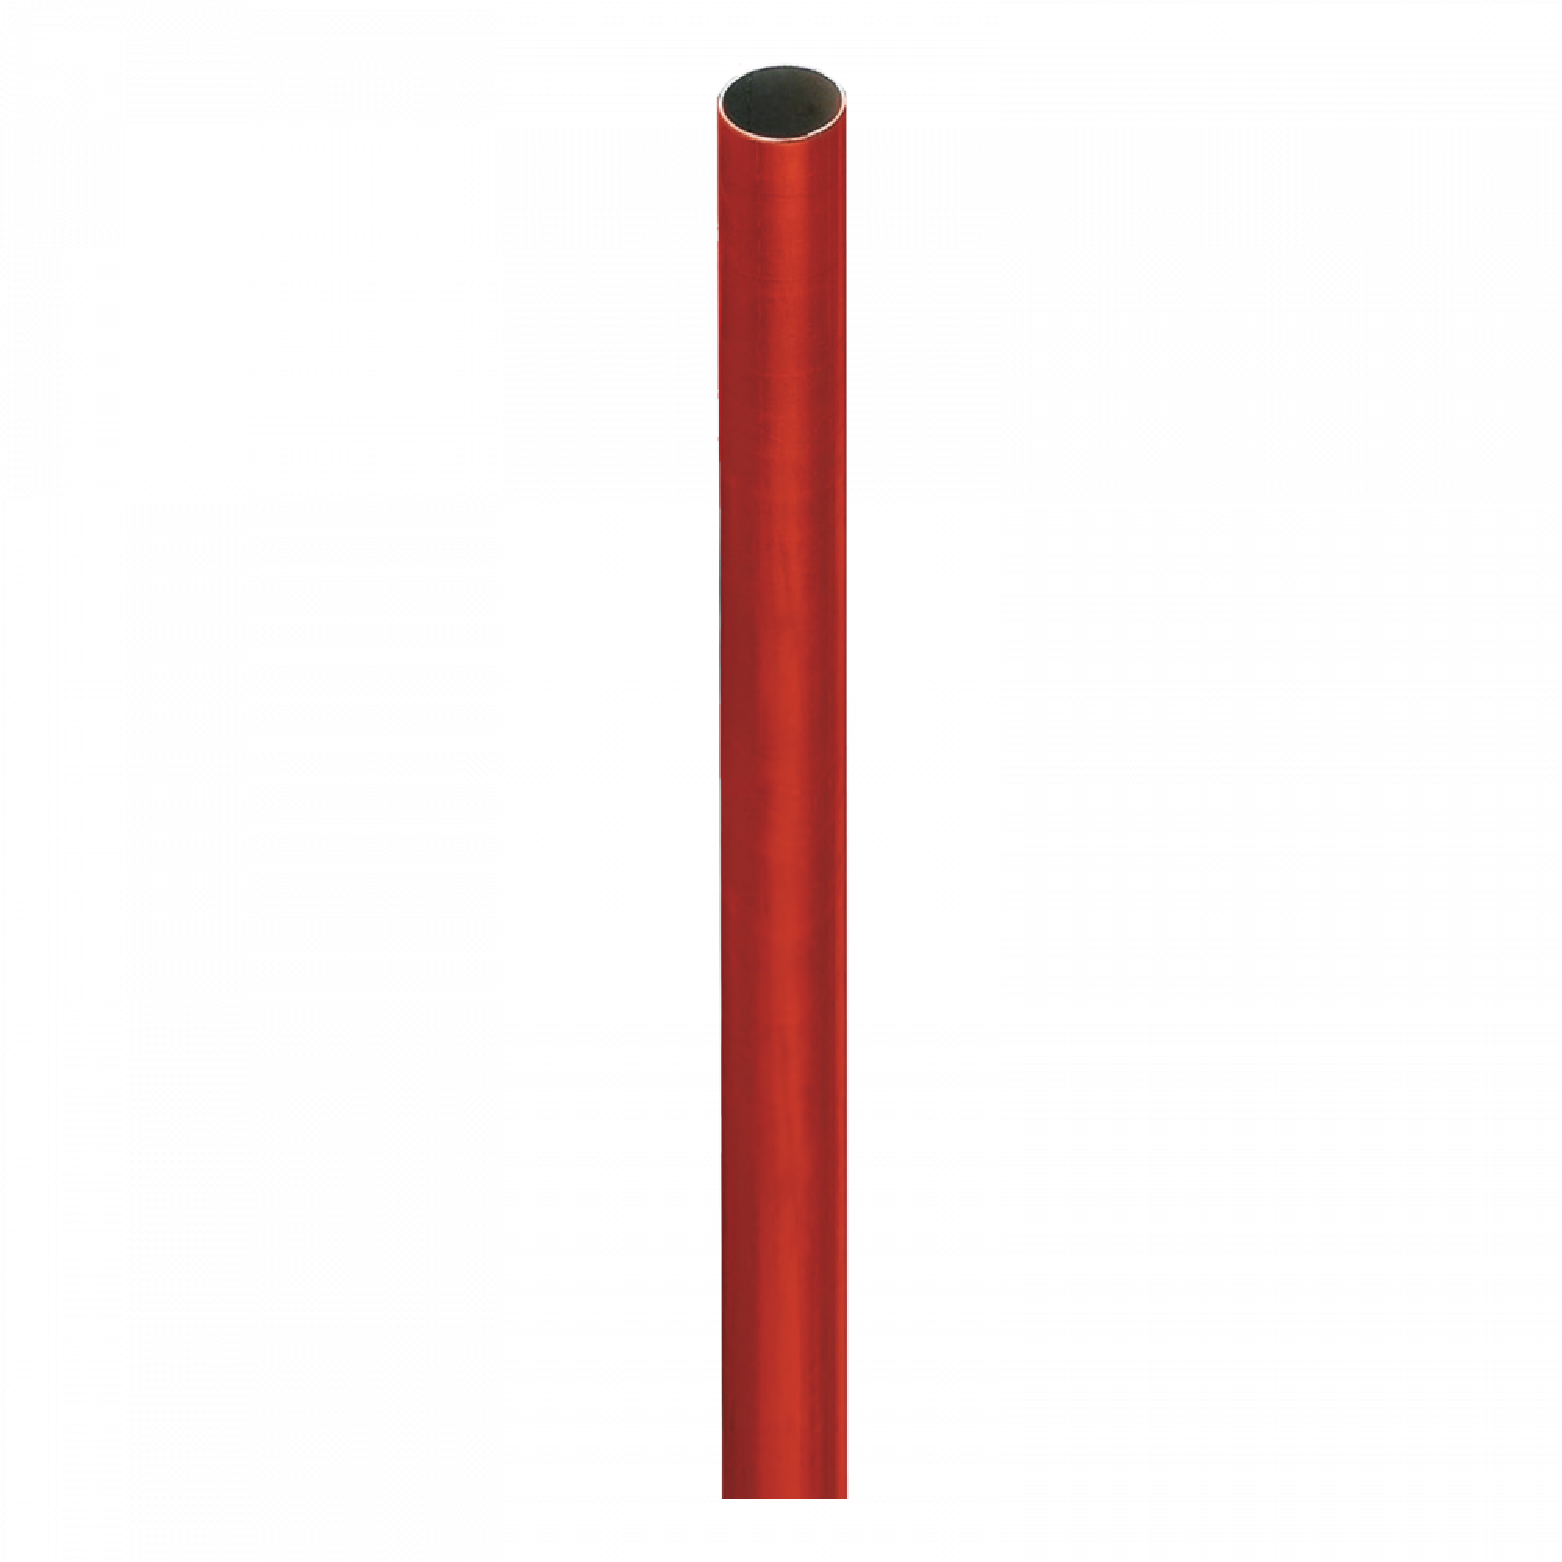
\includegraphics[width=10cm]{img/mastil.pdf}
	\caption{Mástil de acero galvanizado}
	\label{fig:mastil}
\end{figure}

El modelo elegido tiene la referencia 3010 del catálogo de televes. Como se aprecia en la figura \ref{fig:mflector}, el mástil tiene un momento flector
\begin{equation}\label{momentoflector}
\textbf{$M_f =  656.75 \frac{N}{m}$}
\end{equation}, 

\begin{figure}[h!]
	\centering
	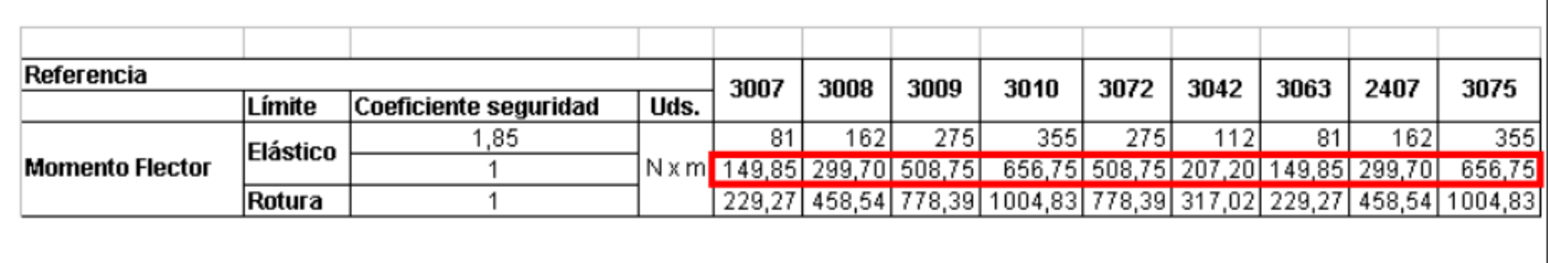
\includegraphics[width=17cm]{img/momentos_flectores.pdf}
	\caption{Momentos Flectores Televés}
	\label{fig:mflector}
\end{figure}


\subsection{Soportes}
Para evitar el contacto con el tejado, dicho mástil irá fijado a la pared del casetón del edificio mediante dos soportes realizados con perfil de hierro que se anclarán al edificio con tacos metálicos de expansión \url{https://www.televes.com/es/240410-soporte-recto-con-perfil-en-u-300mm.html}. La description del soporte se puede encontrar en la figuras \ref{fig:soporte_pared1} así como una foto de la misma en la figura \ref{fig:soporte_pared2}   

\subsection{Anclajes}
Fijación de las dos garras a la pared exterior de la caseta por medio de 4 tacos (8 en total) metálicos de expasión Noutac M6x45 con una carga de extracción de 303Kg.

\begin{figure}[h!]
	\centering
	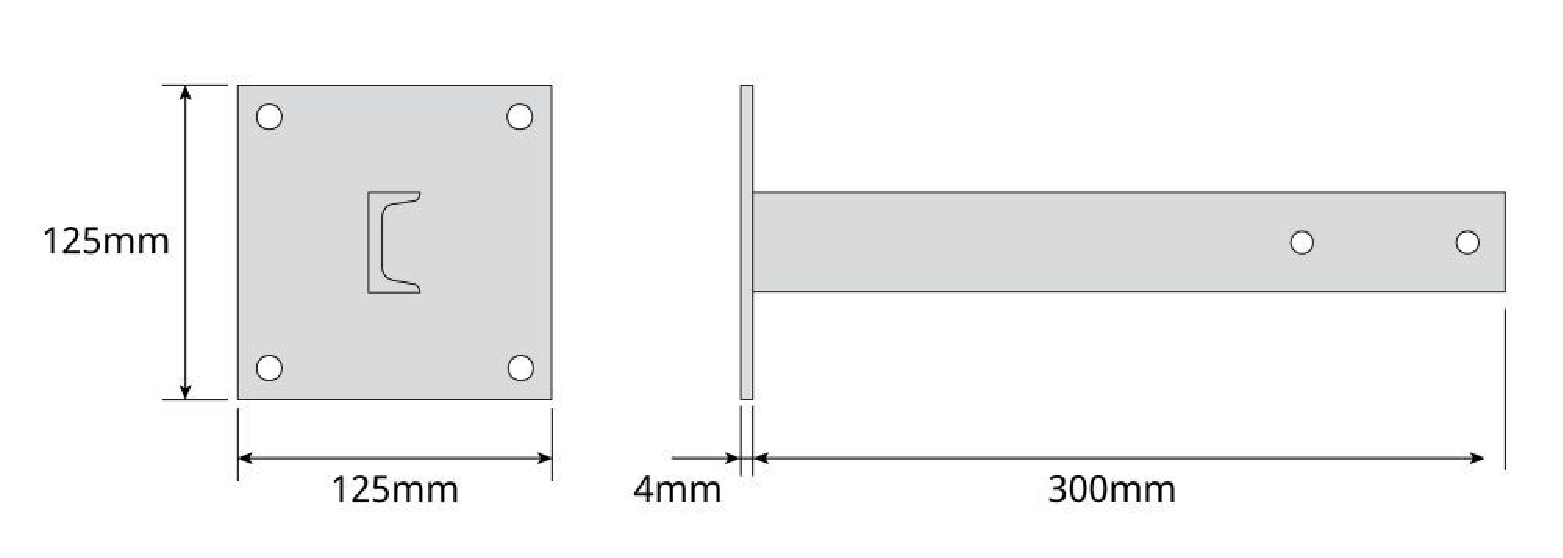
\includegraphics[width=10cm]{img/soporte_pared1.pdf}
	\caption{Descripción de soporte recto}
	\label{fig:soporte_pared1}
\end{figure}

\begin{figure}[h!]
	\centering
	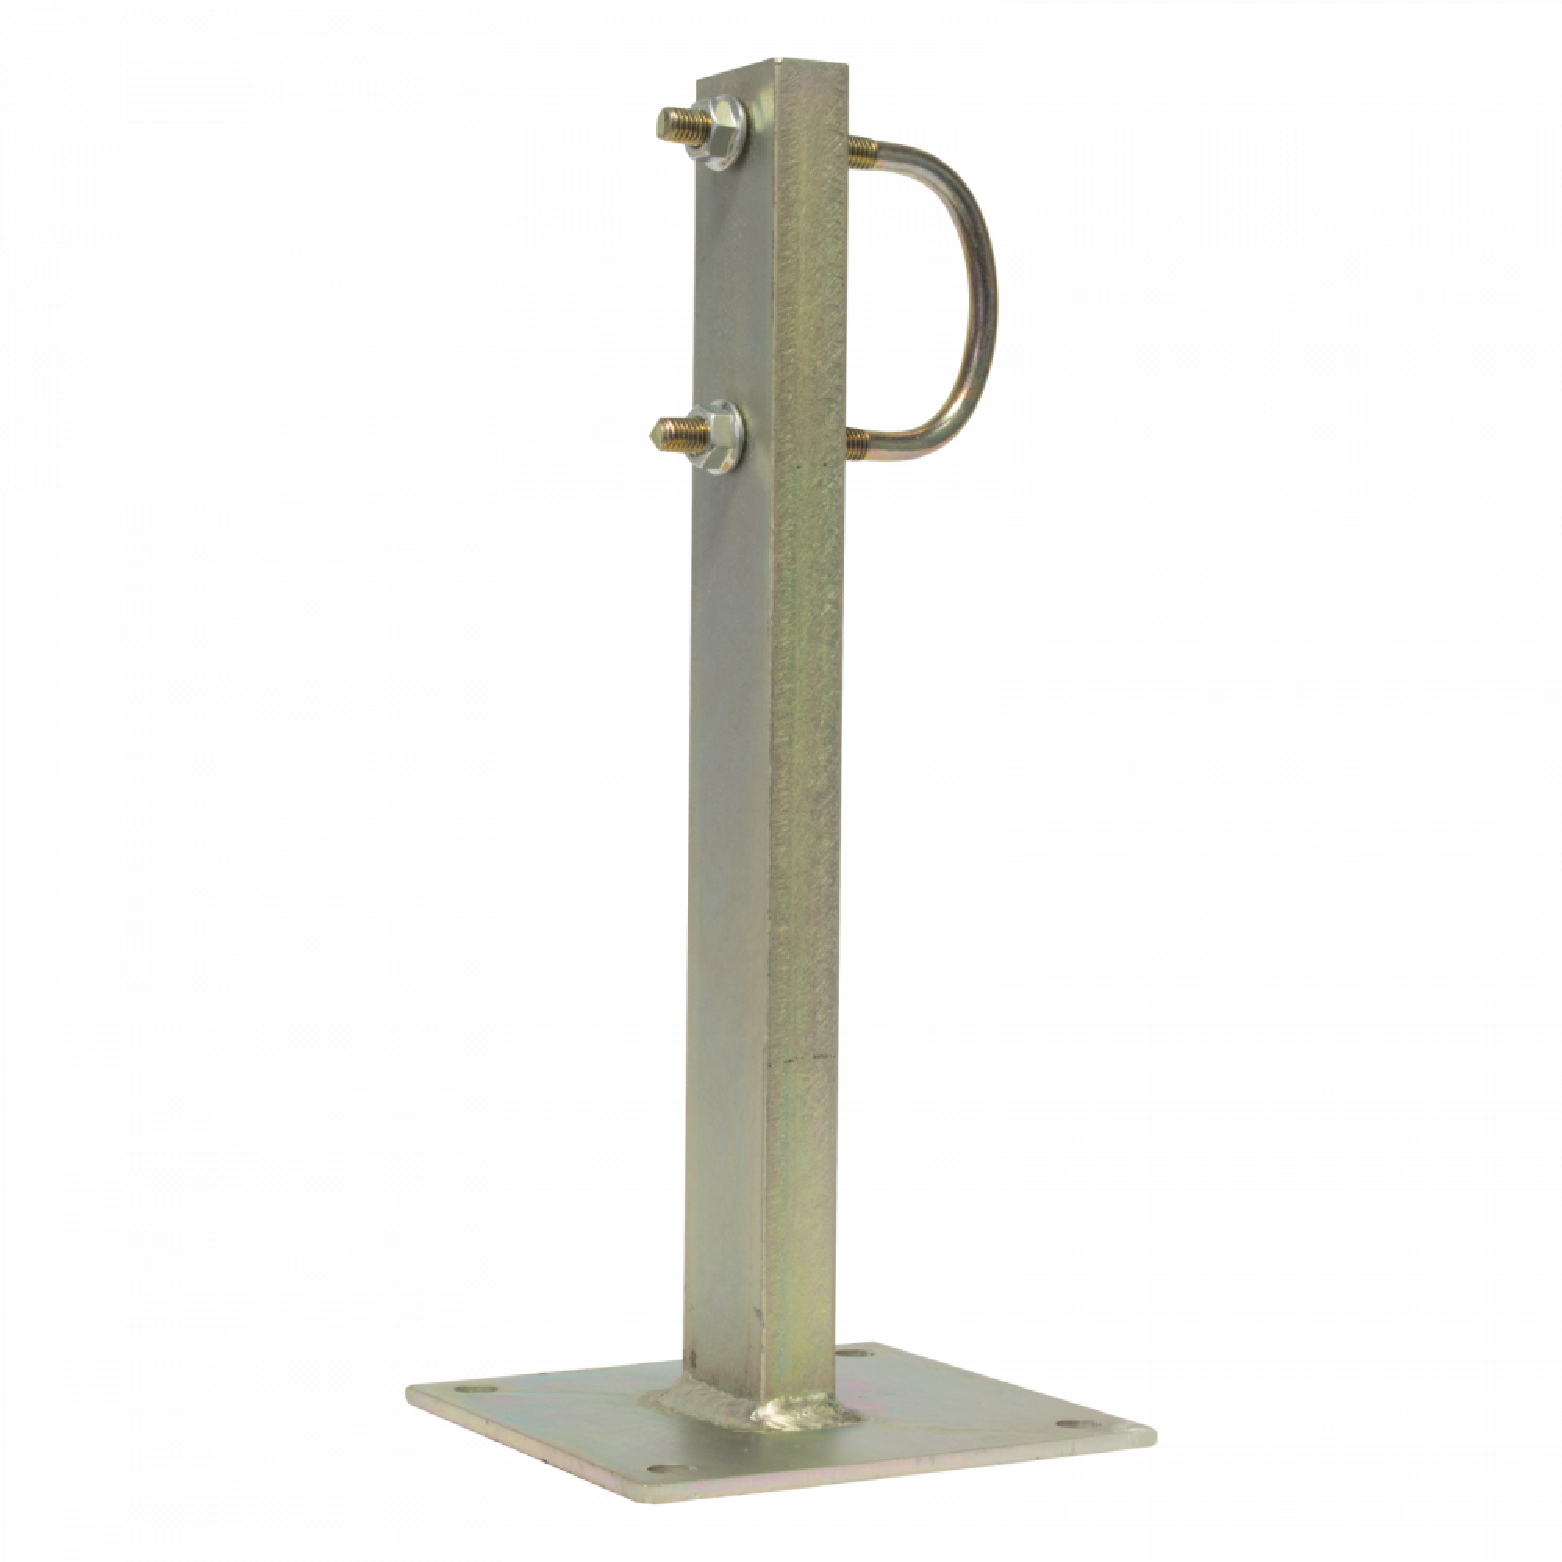
\includegraphics[width=10cm]{img/soporte_pared2.pdf}
	\caption{Soporte recto con perfil en U}
	\label{fig:soporte_pared2}
\end{figure}

\subsection{Mordazas}
La unión entre el soporte y el mástil se realizara mediante dos mordazas para asegurar la estabilidad del mismo. Dichas mordazas son unas TELEVES con referencia 4951, \url{https://www.televes.com/es/mordaza-mastil-zincrpr-mordaza-para-mastil-o-25-45mm.html}. En las figura \ref{fig:mordaza1}, \ref{fig:mordaza2}, se puede ver el detalle de la misma.

\begin{figure}[h!]
	\centering
	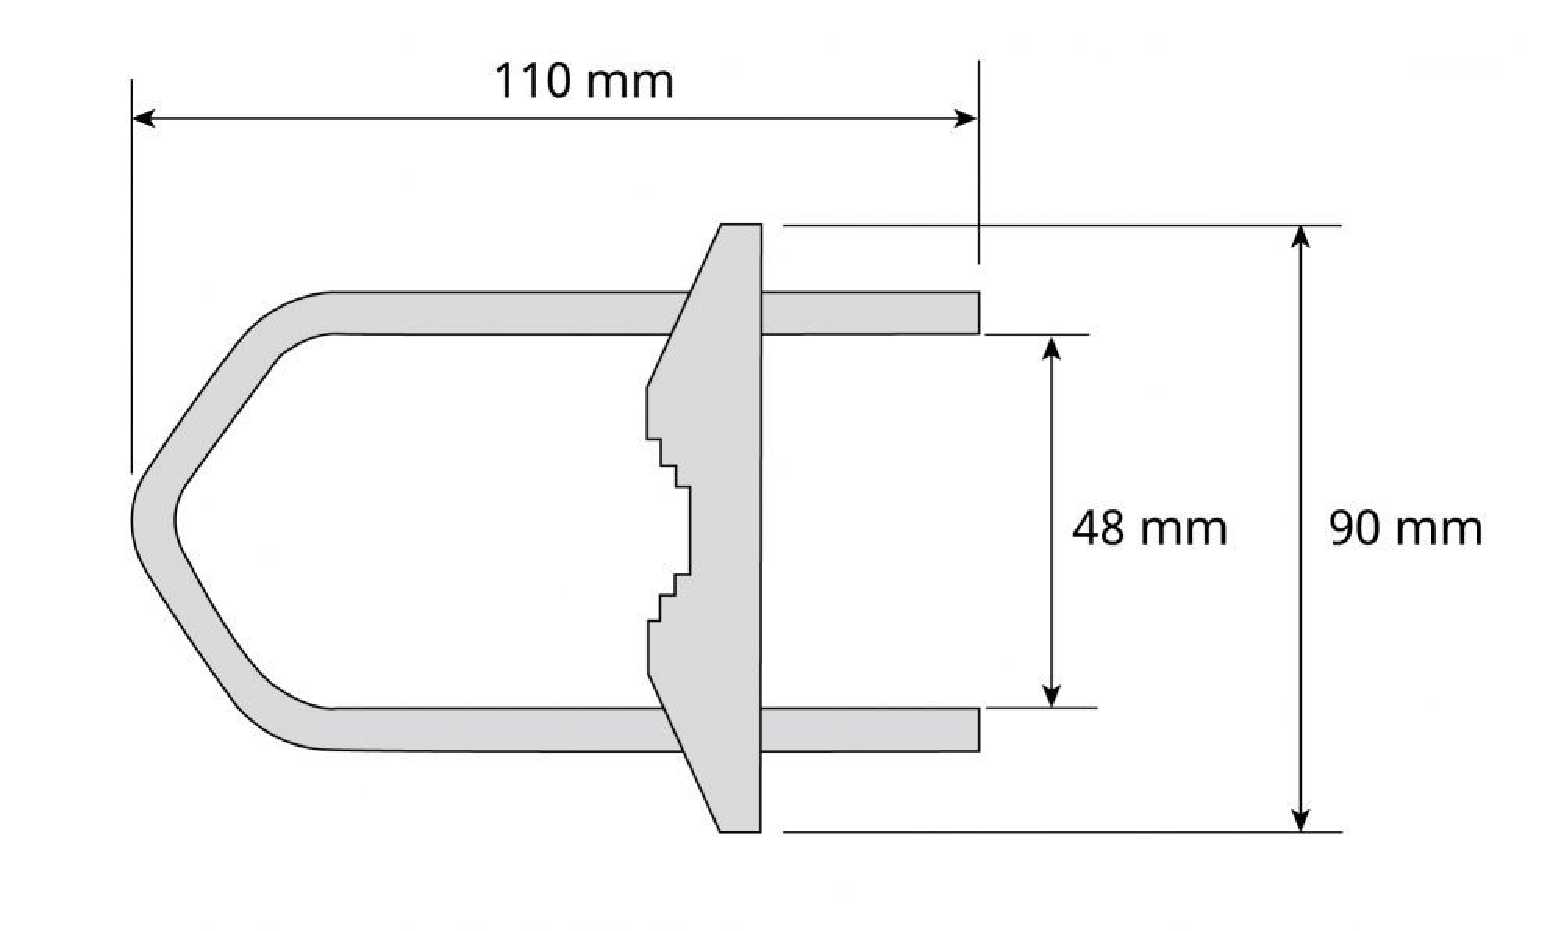
\includegraphics[width=10cm]{img/mordaza1.pdf}
	\caption{Descripción mordaza}
	\label{fig:mordaza1}
\end{figure}

\begin{figure}[h!]
	\centering
	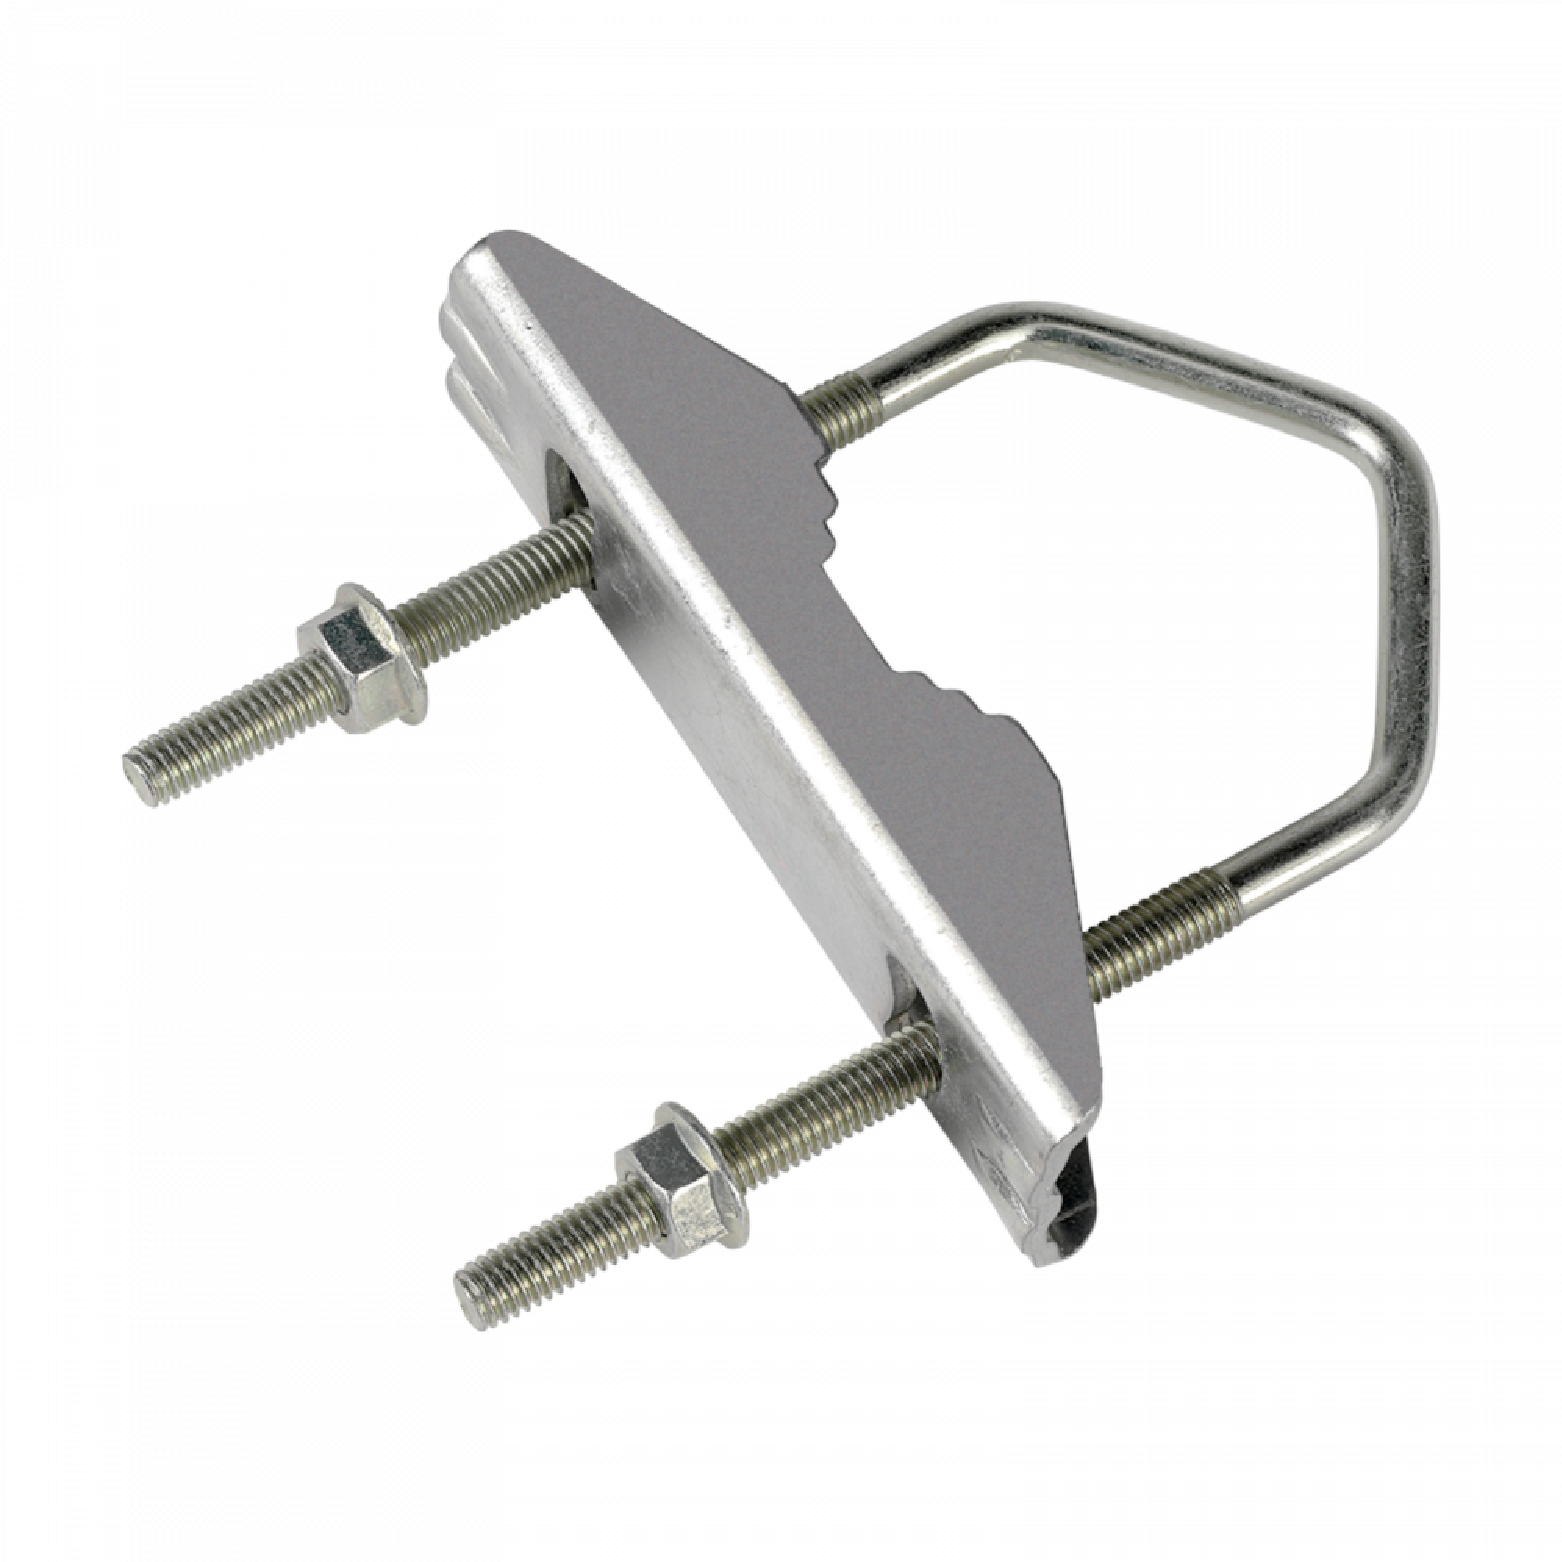
\includegraphics[width=10cm]{img/mordaza2.pdf}
	\caption{Mordaza}
	\label{fig:mordaza2}
\end{figure}


También en color azul se indica la posición de las antenas dipolo que serán arriostradas mediante hilo de nylon coun un diametro de 4mm y fijadas a los muros laterales del edificio mediante tensores adecuados, ver figura adjunta o similares.

Al mástil irán fijadas las antenas VHF/UHF y la antena discono por medio de dos separadores TELEVES ref 3016 y abrazaderas ref. 2067.

\subsection{Antena discono Diamond D3000}

Sobre el mástil se colocará una antena discono diamond d3000 con las siguientes características:
\begin{itemize}
	\item Rango de frecuencias: 25MHz a 3000MHz
	\item Potencia máxima de emisión: bandas de los 50mhz (20.w), 144, 430, 904.y 1200.mhz (200.w)
	\item Ganancia: 2 dB nominal
	\item Longitud: 1.7m
	\item Material de construcción: Aluminio y acero inoxidable
	\item Peso: 1 Kg
	\item Conector: N Hembra
	 
\end{itemize}

Como se puede ver en la figura \ref{fig:antena}

\begin{figure}[h!]
	\centering
	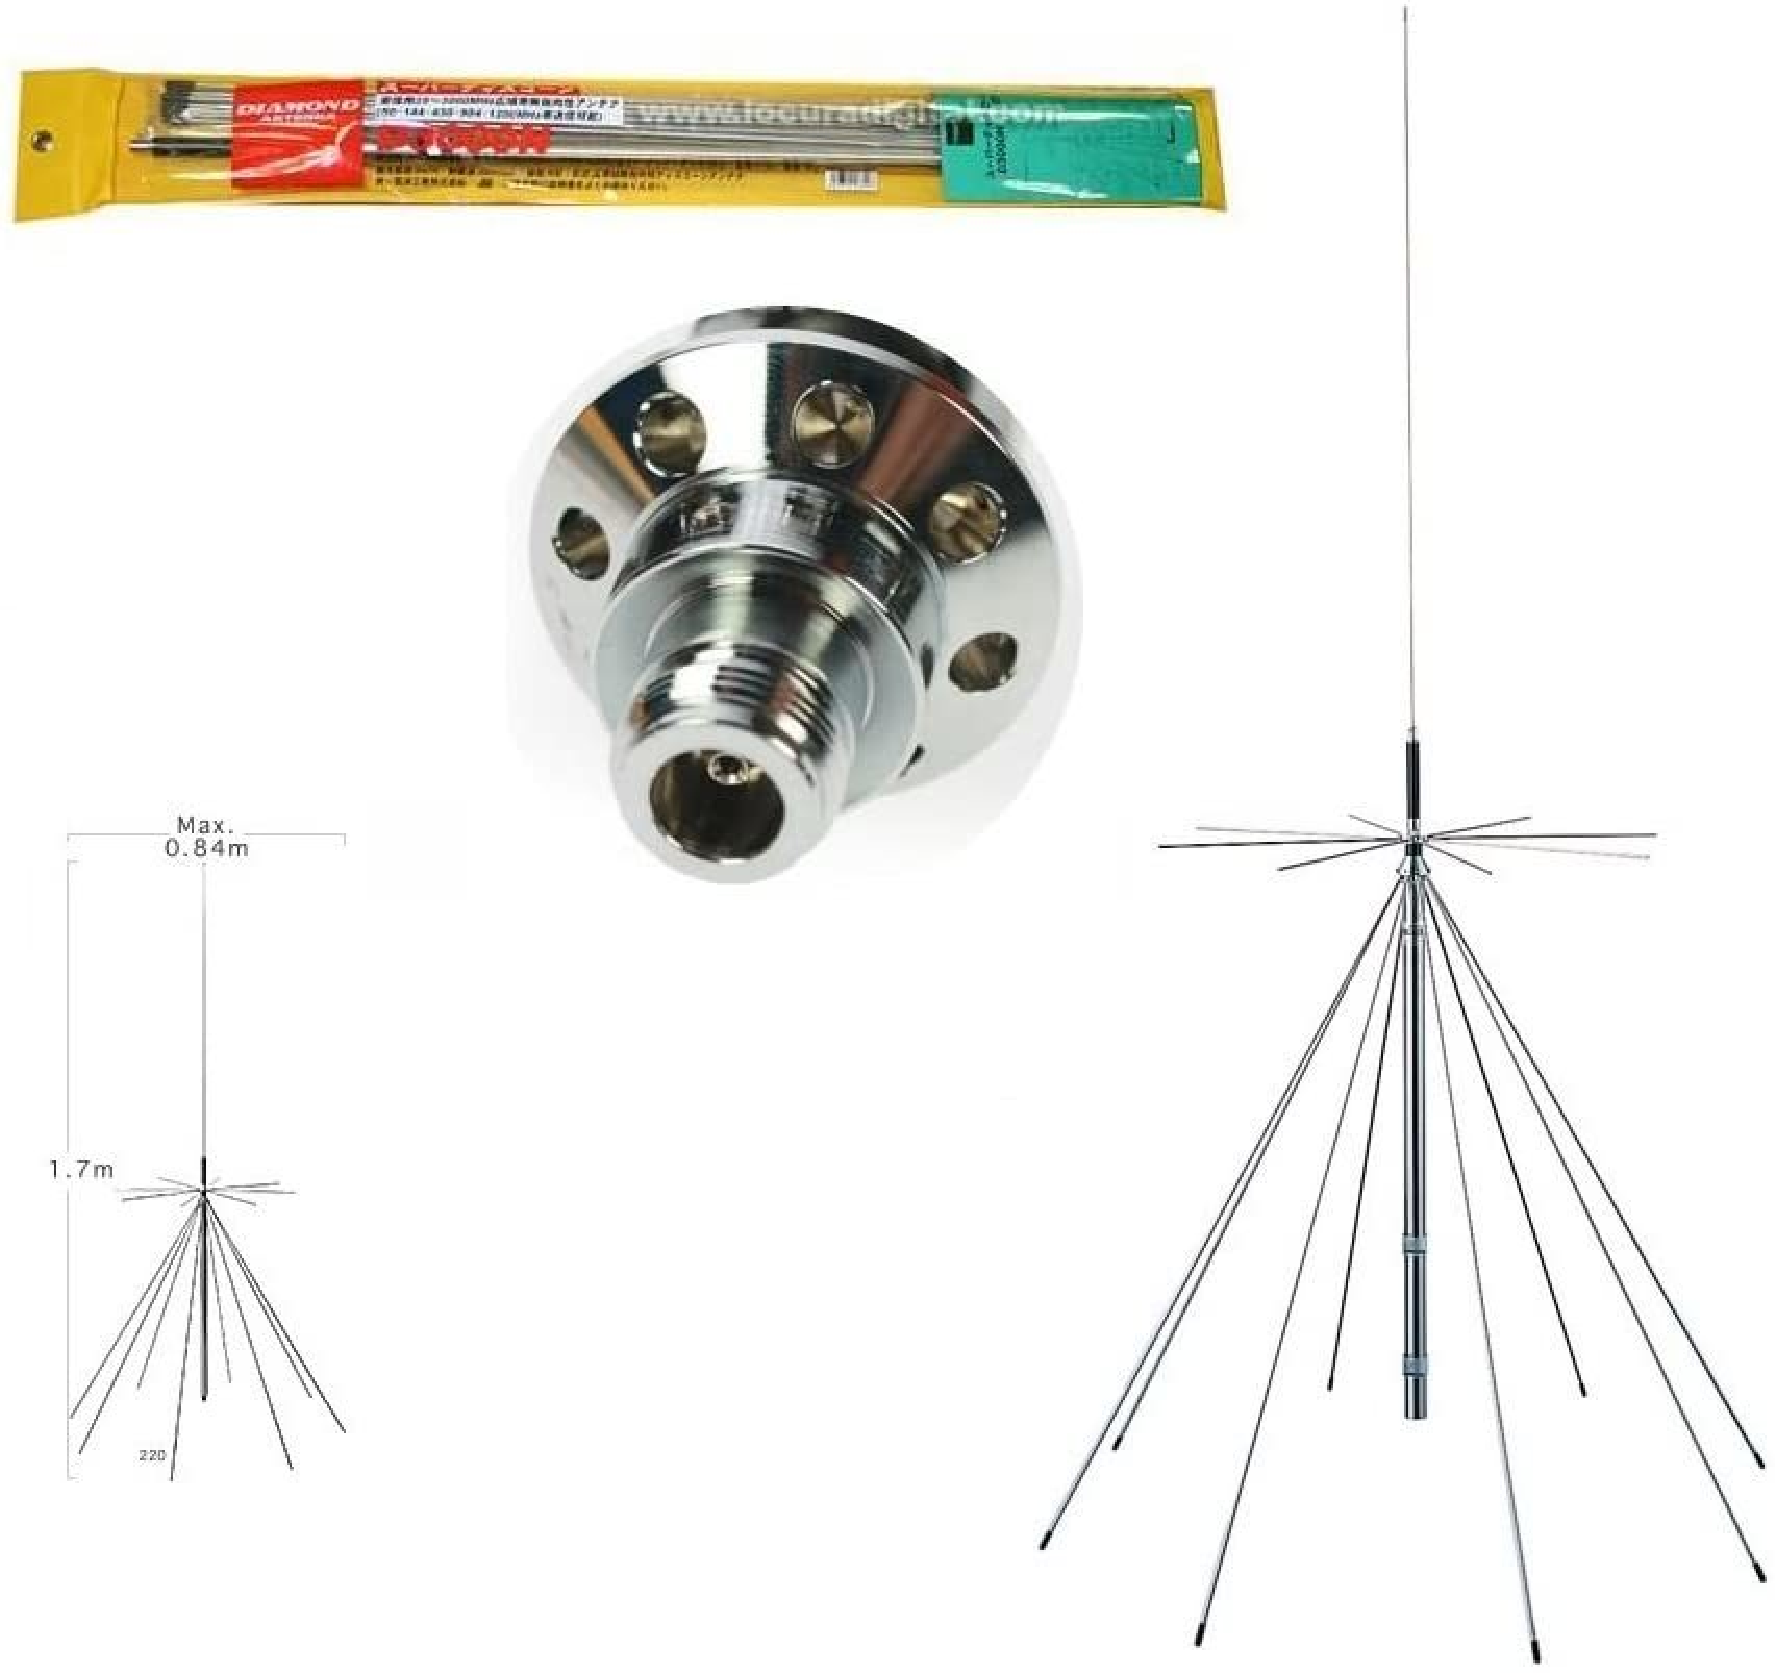
\includegraphics[width=10cm]{img/diamond_d3000.pdf}
	\caption{Antena dicono}
	\label{fig:antena}
\end{figure}

\subsection{Antena Dipolo}
El dipolo aprovechará el mástil para su punto central. Las características del dipolo son las siguientes:
\begin{itemize}
	\item Rango de Frecuencias: 3.5MHz, 7Mhz, 14MHz, 21MHz y 28 Mhz
	\item Longitud: 19.9m
	\item Peso: 2.4Kg
	\item Potencia máxima de emisión: 500 watts (PEP)
\end{itemize}

Como se puede ver en la figura \ref{fig:dipolo}

\begin{figure}[h!]
	\centering
	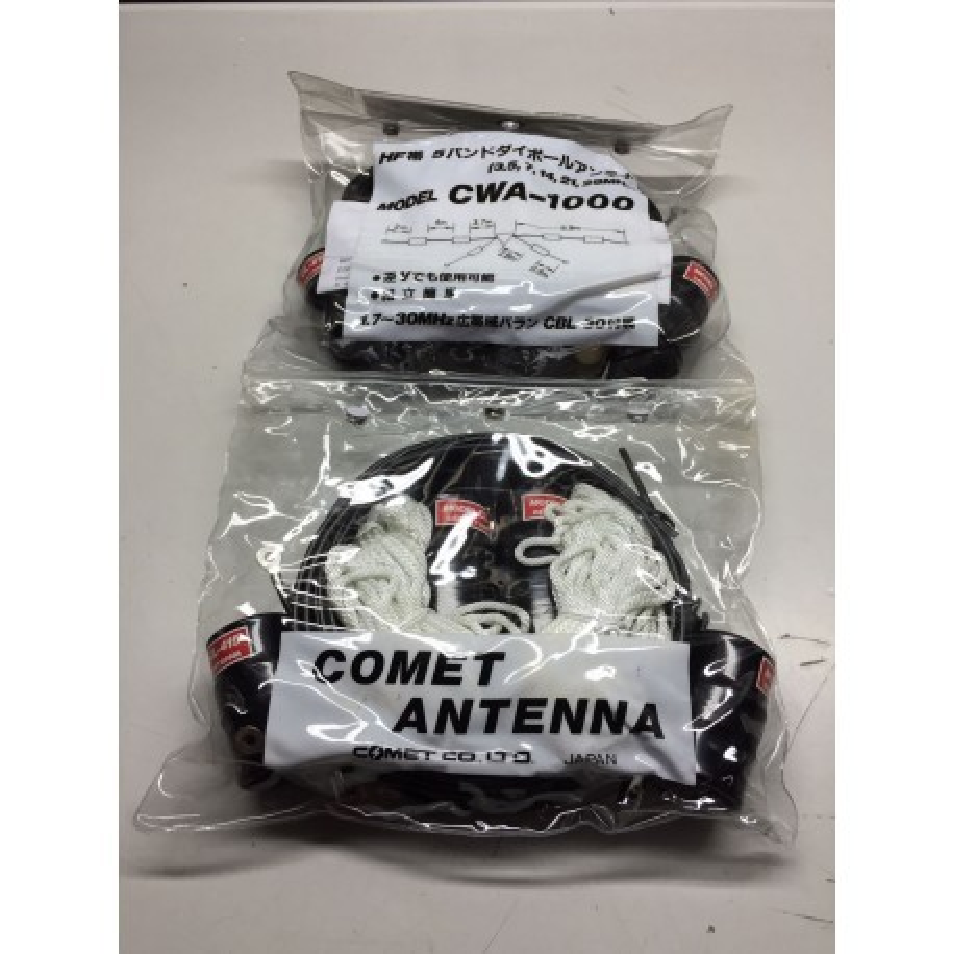
\includegraphics[width=10cm]{img/cwa-1000.pdf}
	\caption{Antena Dipolo}
	\label{fig:dipolo}
\end{figure}


\newpage

\section{Cálculo de la resistencia del viento del conjunto de antenas.}

Para el cálculo de las resistencias, me he basado en los artículos escritos por Diego Doncel \cite{EA1CN}.

Consideraremos la presión del viento P, Normas VDE 0855 parte 1/7.71, más de 20m de altura del edificio. 
A $150 Km/h$, $110 Kg/m^2$ $\rightarrow$ $1080 N/m^2$.
Para los cálculos que siguen, eligiré un valor más conservador para una máyor seguridad, $1100 N/m^2$. 


Definimos: 
\begin{itemize}
	\item Superficie equivalente, $S_{eq}$
	\item Resistencia al viento, $R_{w}$.
\end{itemize}

\subsection{Antena discono.}

\begin{eqnarray}
\text{8 Radiales superiores:} S_{eq} &=& 8 * 0.28m * 0.005m = 0.0112m^{2} \\
\text{8 Radiales inferiores:} S_{eq} &=& 8 * 0.820m * 0.005m = 0.0328m^{2}\\
\text{Eje de la antena:} S_{eq} &=& 1.7m * 0.05m = 0.085m^{2} \\
S_{eq}  \text{total}  &=& 0.0112m^{2} + 0.0328m^{2} +  0.085m^{2} = 0.129m^{2} \\
R_{w} &=& 1100N/m^{2} * 0.129m^{2} = 142N
\end{eqnarray}

\subsection{Dipolo multibanda.}
Calculamos su resistencia al viento, teniendo en cuenta el peso del conjunto.
\begin{eqnarray}
R_{w} &=& 2.5Kg * 9.8 = 24.5N 
\end{eqnarray}


\subsection{Mástil.}
Como hemos visto en \ref{momentoflector}, el momento flector del mástil es de $M_f = 656.75 \frac{N}{m}$

El momento flector de la antena lo calculamos de la siguiente forma
\begin{eqnarray}
M_{kgm} &=& d x F_{total}  \\
\text{longitud del voladizo: } d & = & 2.5m \\
\text{Fuerza Antena Dicono: } F_{dcn} &=& 142N \\
\text{Fuerza Dipolo: } F_{dpl} &=& 24.5 \\
\text{Fuerza Total: } F_{total} &=& F_{dcn} + F_{dpl} = 166.5N \\
M_{kgm} &=& 166.5 x 2.5 = 416.2N
\end{eqnarray}

Quedando securizada la instalación siendo menor el momento flector del conjunto de la antena, $416.2N$ que el momento flector soportado por el mástil, $656.75N$.

\newpage

\section{Legislación municipal aplicable - Comunidad de Madrid -.}
\includepdf[pages=7-8]{anexos/normativa}
\newpage

\section{R.D. 2623/86 capítulo IV. Prescriciones técnicas de las antenas y sus elementos anejos.}
\includepdf[pages=7-8]{anexos/BOE}
\newpage

\section{Anexos}
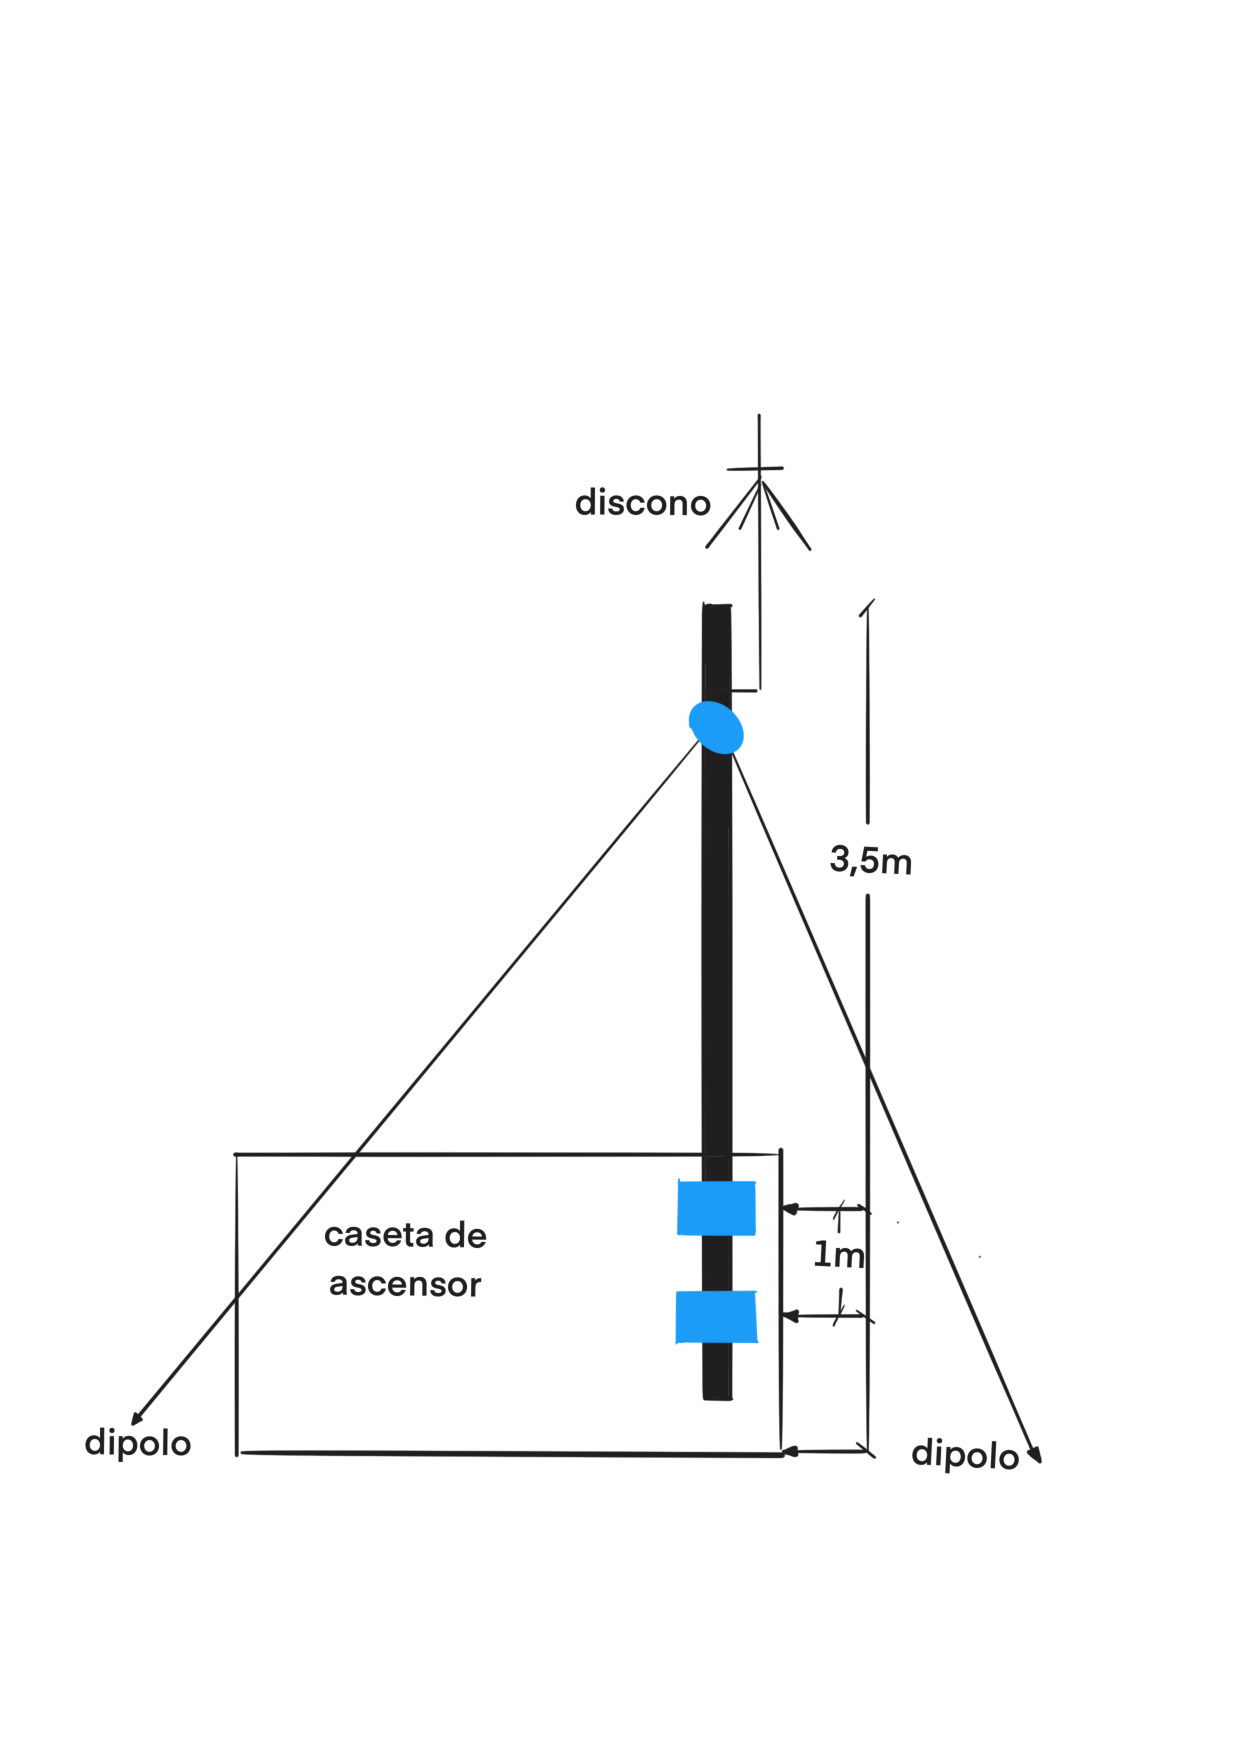
\includepdf{anexos/anclajes}
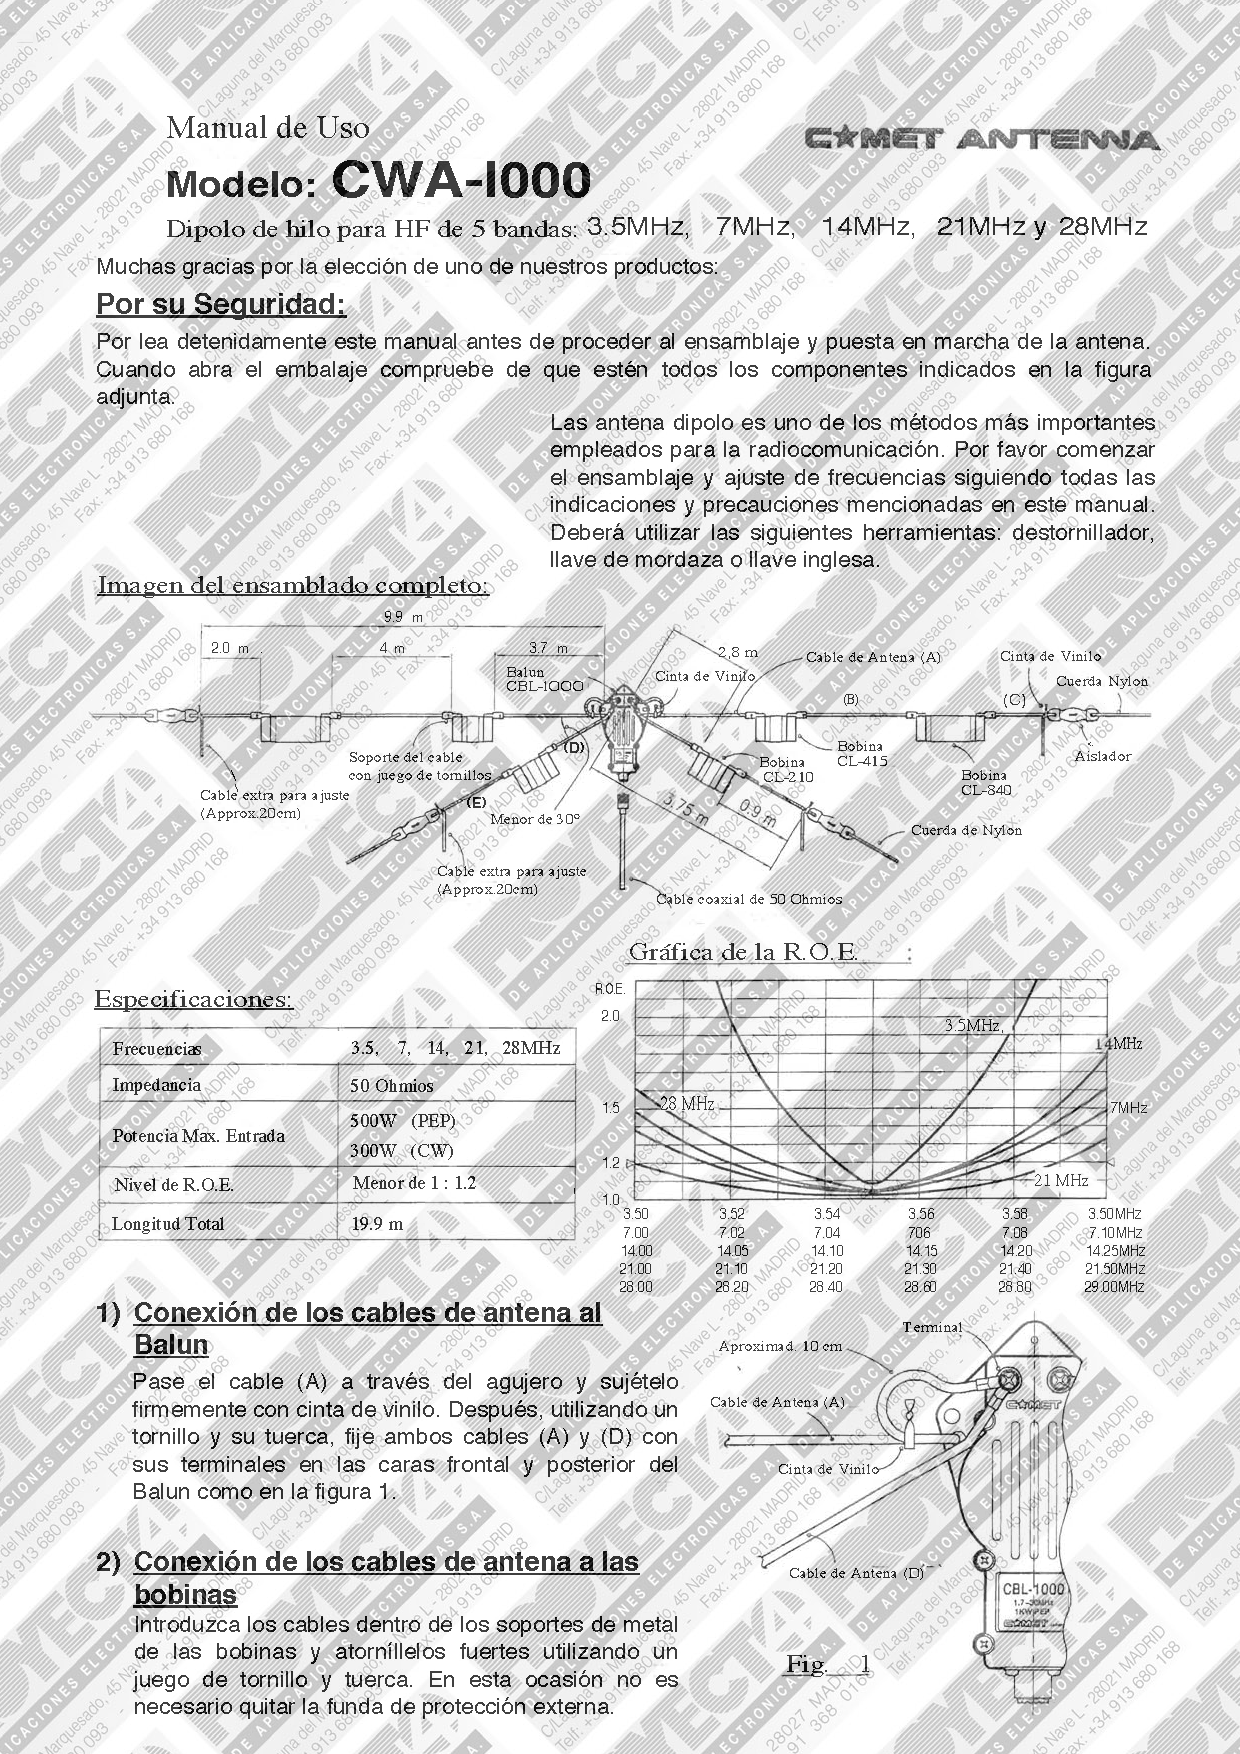
\includepdf{anexos/CWA-1000}
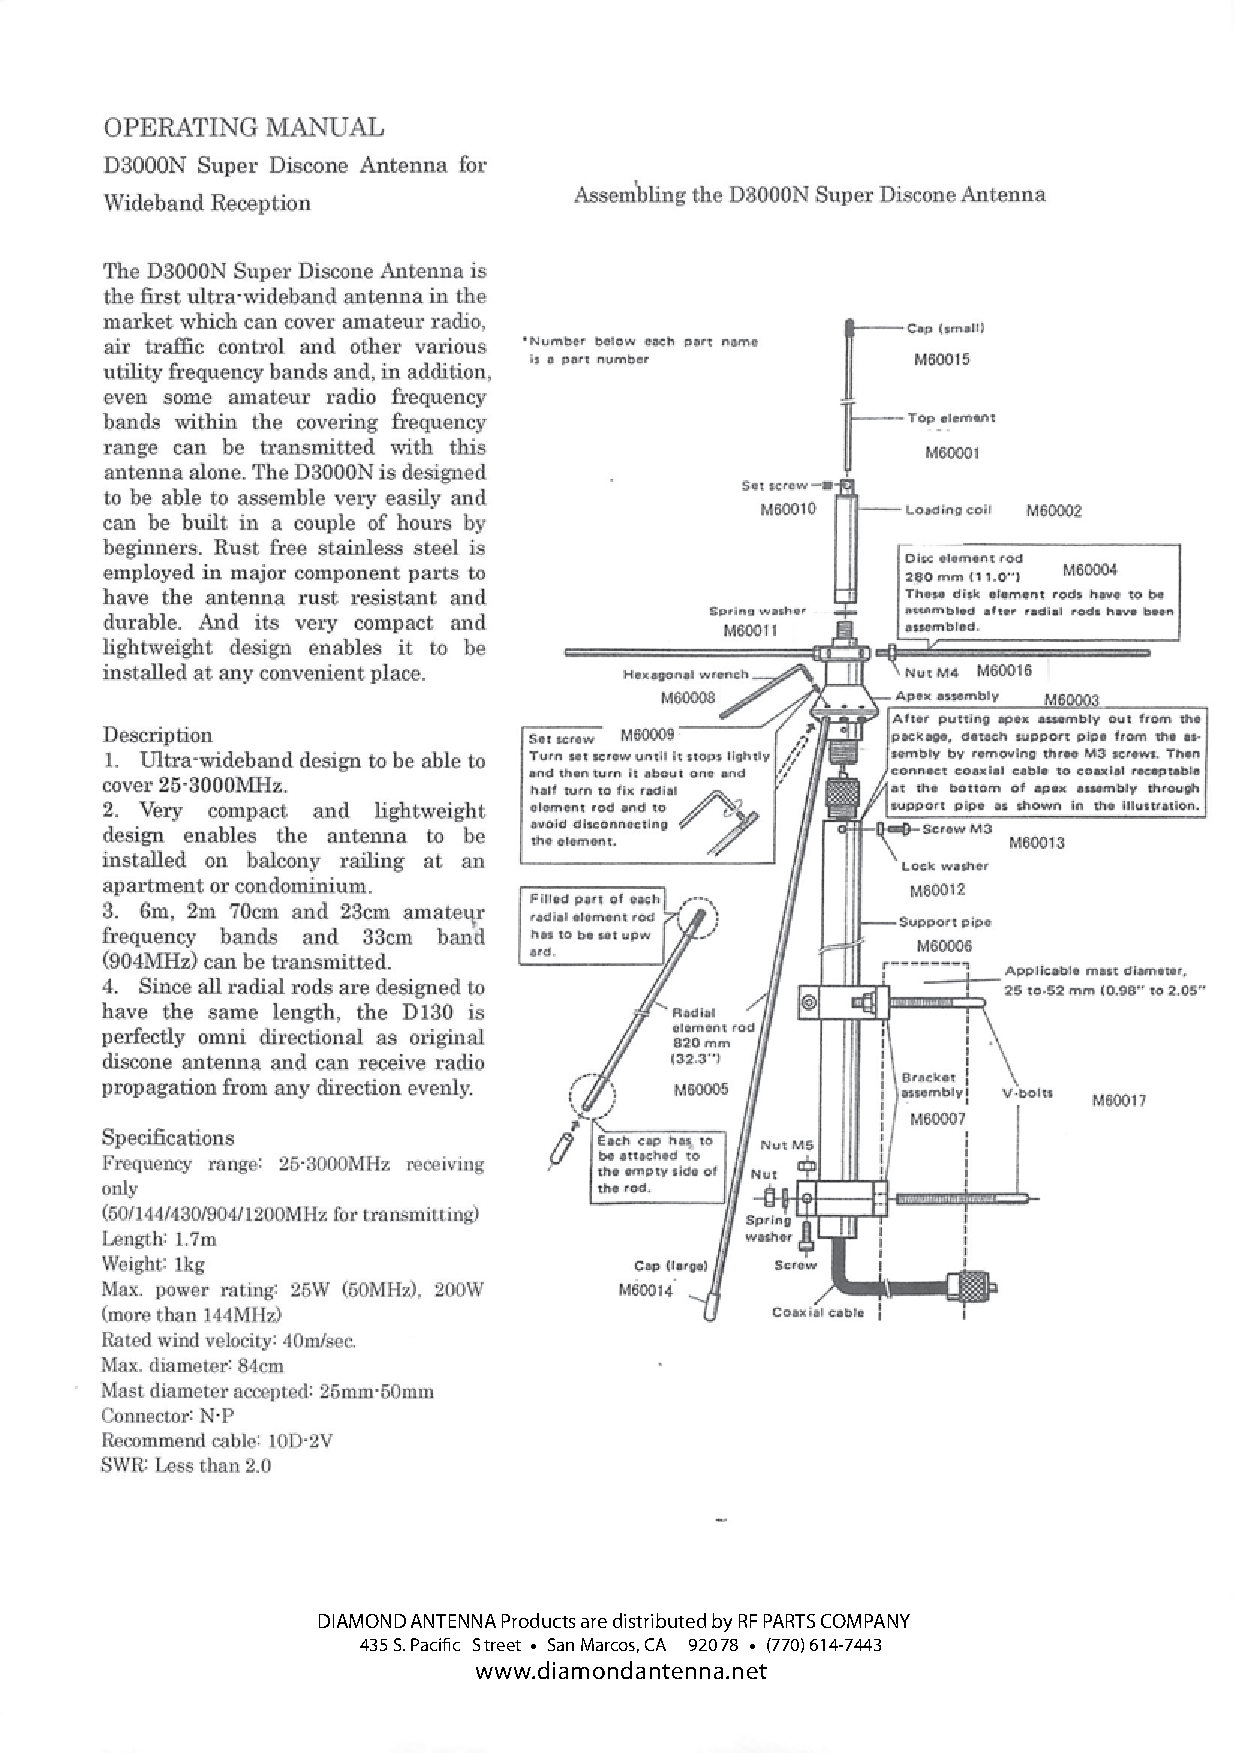
\includepdf{anexos/D3000N}
\newpage

\section{Memoria técnica solicitudes tipo 6.}
\newpage

\section{Bibliografía}
\begin{thebibliography}{0}
	\bibitem{EA1CN} Diego Doncel, EA1CN. Revista URE Noviembre 2017. Montaje de antenas (I,II, III, IV).
\end{thebibliography}

\end{document}
